\documentclass[crop,tikz,convert={outext=.svg,command=\unexpanded{pdf2svg \infile\space\outfile}},multi=false]{standalone}[2012/04/13]

\usepackage[utf8]{inputenc}
\usepackage{amsmath, amssymb}
\usepackage{pgfplots}


%-------------------------------------
% Tikz and pgf options & definitions
%-------------------------------------
\pgfplotsset{compat=1.15}
\pgfmathsetseed{1}

\usetikzlibrary{positioning}
\usetikzlibrary{shapes}
\usetikzlibrary{backgrounds, fit}
\usetikzlibrary{calc}
\usetikzlibrary{decorations.markings}
\usetikzlibrary{matrix}

\def\colorvector at (#1,#2,#3){
\coordinate (A) at (#1, #2);
\filldraw[draw=black,fill=test!!+] (A)++(0,0) rectangle ++(0.25,0.25) node (A0) {};
\filldraw[draw=black,fill=test!!+] (A)++(0.3,0) rectangle ++(0.25,0.25) node (A1) {};
\filldraw[draw=black,fill=test!!+] (A)++(0.6,0) rectangle ++(0.25,0.25) node (A2) {};
\node[right=of A2, xshift=-7.5ex, yshift=-0.75ex] {$\ldots$};
\filldraw[draw=black,fill=test!!+] (A)++(1.5,0) rectangle ++(0.25,0.25) node (A4) {};
\node[left=of A1, xshift=4.4ex, yshift=-0.75ex] (BEG\i) {$#3=[$};
\node[right=of A4, xshift=-8ex, yshift=-0.75ex] (END\i) {$]^{T}$};
}

\begin{document}
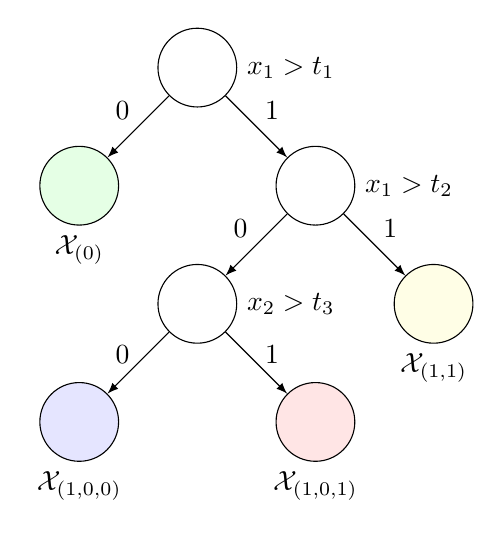
\begin{tikzpicture}[
edge from parent/.style={draw,-latex},
level distance=15mm,
level 1/.style={sibling distance=30mm},
level 2/.style={sibling distance=30mm},
level 3/.style={sibling distance=30mm},
level 4/.style={sibling distance=15mm}
]

\usetikzlibrary{shapes}
\tikzstyle{c} = [draw, shape=circle,minimum width=10mm]
\tikzstyle{r} = [draw, shape=rectangle,minimum width=10mm]
\tikzstyle{tr} = [draw,isosceles triangle, shape border rotate=90, anchor=north]
\node[c, label=right:{$ x_{1} > t_{1} $}]{}[edge from parent]
    child {node[c, fill=green!10, label=below:{$ {\cal X}_{\left( 0 \right)} $}] {}
        edge from parent coordinate (ea);
    }
    child {node[c, label=right:{$ x_{1} > t_{2} $}]{}
        child {node[c, label=right:{$ x_{2} > t_{3} $}]{}
            child{node[c, fill=blue!10, label=below:{$ {\cal X}_{\left( 1, 0, 0 \right)} $}]{}
                edge from parent coordinate (e14);
            }
            child{node[c, fill=red!10, label=below:{$ {\cal X}_{\left( 1, 0, 1 \right)} $}]{}
                edge from parent coordinate (e16);
            }
            edge from parent coordinate (e30);
        }
        child {node[c, fill=yellow!10, label=below:{$ {\cal X}_{\left( 1, 1 \right)} $}]{}
            edge from parent coordinate (e25);
        }
        edge from parent coordinate (e55);
    };
\node at([xshift=-2mm,yshift=2mm]ea)  {0};
\node at([xshift=2mm,yshift=2mm]e55) {1};
\node at([xshift=2mm,yshift=2mm]e25) {1};
\node at([xshift=-2mm,yshift=2mm]e30) {0};
\node at([xshift=-2mm,yshift=1mm]e14) {0};
\node at([xshift=2mm,yshift=1mm]e16) {1};
\end{tikzpicture}
\end{document}